



\thispagestyle{fancy}
	
	%\vspace{-2em} % Adjust vertical space as needed
% 	\begin{center}



% \addcontentsline{toc}{subsection}{Message of the Vice Chancellor}    
% \subsection*{\textsc{Message of the Vice Chancellor}}
% 	\end{center}

   
    
%     \begin{wrapfigure}{l}{0.3\textwidth}
% 		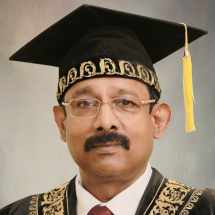
\includegraphics[width=0.3\textwidth]{Images/VC.png}
% 	\end{wrapfigure}
	%\vspace{2em} % Adjust vertical space as needed

\addmessage{Vice Chancellor}{VC.jpeg}


	
	
	I am delighted to join you for the 8\textsuperscript{th} International Research Symposium (IRS 2024) of the University of Vocational Technology, focused on the timely and transformative theme of 'Vocational Education for a Sustainable Greener Economy.' This event is a powerful testament to the university's commitment to leveraging research and education to drive sustainable development.
    
In today’s world, the role of Technical and Vocational Education and Training (TVET) has never been more significant. As economies across the globe pivot towards sustainability and green practices, TVET emerges as a critical driver of this transition. By equipping individuals with the skills and knowledge needed to tackle environmental and economic challenges, this sector not only empowers communities but also lays the foundation for a resilient and prosperous future. 

The University of Vocational Technology leads this transformative journey by seamlessly integrating innovative education with practical applications to advance sustainable development goals. Its unwavering commitment to research and development spans critical areas such as Educational Strategies for Sustainable TVET, Engineering Technology for a Green Economy, Digital Technologies and Creative Industries, Innovation and Entrepreneurship for Economic Resilience, and Sustainable Practices for a Multifunctional Green Economy. These initiatives highlight the essential role of education and research in tackling the multifaceted challenges of the 21\textsuperscript{st} century and driving progress toward a more sustainable future.

IRS 2024 provides an invaluable platform for researchers, educators, and industry leaders to collaborate and exchange insights. It is through such dialogues and partnerships that we can chart pathways to ensure vocational education remains relevant, innovative, and impactful.  

As we gather here today, let us reaffirm our collective commitment to sustainability and strive to create a greener, more equitable economy. I extend my heartfelt congratulations to all the authors for your published research work. I would also like to express my heartfelt gratitude to the Organizing Committee, all Reviewers, and the staff of the University of Vocational Technology for their dedicated efforts in making this event a success.   


%	\vspace{1cm}
	\noindent
	Prof. C. Mahesh Edirisinghe\\
	Vice Chancellor
	
	\newpage
	